\documentclass[xcolor=pdftex,dvipsnames,table,mathserif,aspectratio=169]{beamer}
\usetheme{metropolis}
%\usetheme{Darmstadt}
%\usepackage{times}
%\usefonttheme{structurebold}

\usepackage[english]{babel}
%\usepackage[table]{xcolor}
\usepackage{pgf,pgfarrows,pgfnodes,pgfautomata,pgfheaps}
\usepackage{amsmath,amssymb,setspace}
\usepackage[latin1]{inputenc}
\usepackage[T1]{fontenc}
\usepackage{relsize}
\usepackage[absolute,overlay]{textpos} 
\newenvironment{reference}[2]{% 
  \begin{textblock*}{\textwidth}(#1,#2) 
      \footnotesize\it\bgroup\color{red!50!black}}{\egroup\end{textblock*}} 

\DeclareMathSizes{10}{10}{6}{6} 


\title [Switching]{Switching Costs: Handel: Adverse Selection and Inertia in Health Insurance Markets}
\author{C.Conlon }
\institute{Grad IO }
\date{Fall 2020}
\setbeamerfont{equation}{size=\tiny}
\begin{document}

\begin{frame}
\titlepage
\end{frame}

\begin{frame}
\frametitle{Goals of the Paper}

\begin{itemize}
\item Theory Testing

\begin{itemize}
\item Does information provision worsen adverse selection in a
market where consumers face switching costs? Does unraveling result?
\end{itemize}

\item Measurement

\begin{itemize}
\item Identify the value of ``switching costs"
\item Measure consumer welfare change when switching costs fall, given the
\textbf{endogenous} pricing response

\item Measure both adverse selection and risk preferences (including
heterogeneity of risk aversion)
\end{itemize}

\item Methodology

\begin{itemize}
\item Develop non-parametric model linking modeled health risk to
total medical expenditures using observed cost data
\end{itemize}
\end{itemize}
\end{frame}

%--------------------------------------------------------------------------------

\begin{frame}{Handel: Main Idea}
\begin{itemize}
\item There is a tradeoff when introducing an information provision policy in markets
in which adverse selection exists:

\begin{itemize}
\item As ones lowers switching costs, those enrollees with the lowest
costs/lowest risk aversion parameters reallocate and select less
comprehensive coverage

\item Comprehensive plans contain riskier pool; consumers in the pool suffer as premiums
increase due to adverse selection (remaining enrollees in comprehensive plan
have higher costs). ``Death spiral" can occur.
\end{itemize}

\end{itemize}
\end{frame}

%--------------------------------------------------------------------------------

\begin{frame}{Handel: Research Question}
\begin{itemize}
\item For one employer/array of health plans, does a reduction in switching costs harm
social welfare?
\end{itemize}
\end{frame}

%--------------------------------------------------------------------------------

\begin{frame}{Data}
Data from one large, self-insured employer

\begin{itemize}
\item Have employee plan choices, claim-level employee utilization and
expenditure data, employee demographics

\begin{itemize}
\item job char, age, gender, income, job tenure, `quantitatively
sophisticated' manager

\item dependent's type + age/gender
\end{itemize}

\item Focus on a balanced panel of employees

\begin{itemize}
\item must work at the firm from $t_{-1}$ to $t_{1}$

\item enrolled in a PPO in each of these years

\item Excludes employees who enter or exit firm

\begin{itemize}
\item Might these be the type of consumer with lower switching costs? Bias?

\item Decisions of new cohorts could help identification?
\end{itemize}
\end{itemize}
\end{itemize}
\end{frame}

%--------------------------------------------------------------------------------

\begin{frame}
\frametitle{Data}

\begin{itemize}
\item At year $t_{0}$, all enrollees actively select a new plan, with no
default.

\begin{itemize}
\item Switching costs = 0

\item 5 options, 3 PPOs that differ only in financial characteristics (same
network)

\item With no network effects, the switching costs may represent lower bound
\end{itemize}

\item In $t_{1}+$, default is to remain in past choice

\item Plan prices adjust in $t_{1}+$

\item Past claims data (diagnoses + spending); used to construct an ex ante out-of-pocket expense
measure

\end{itemize}
\end{frame}

\begin{frame}{How do insurance contracts look?}
\begin{center}
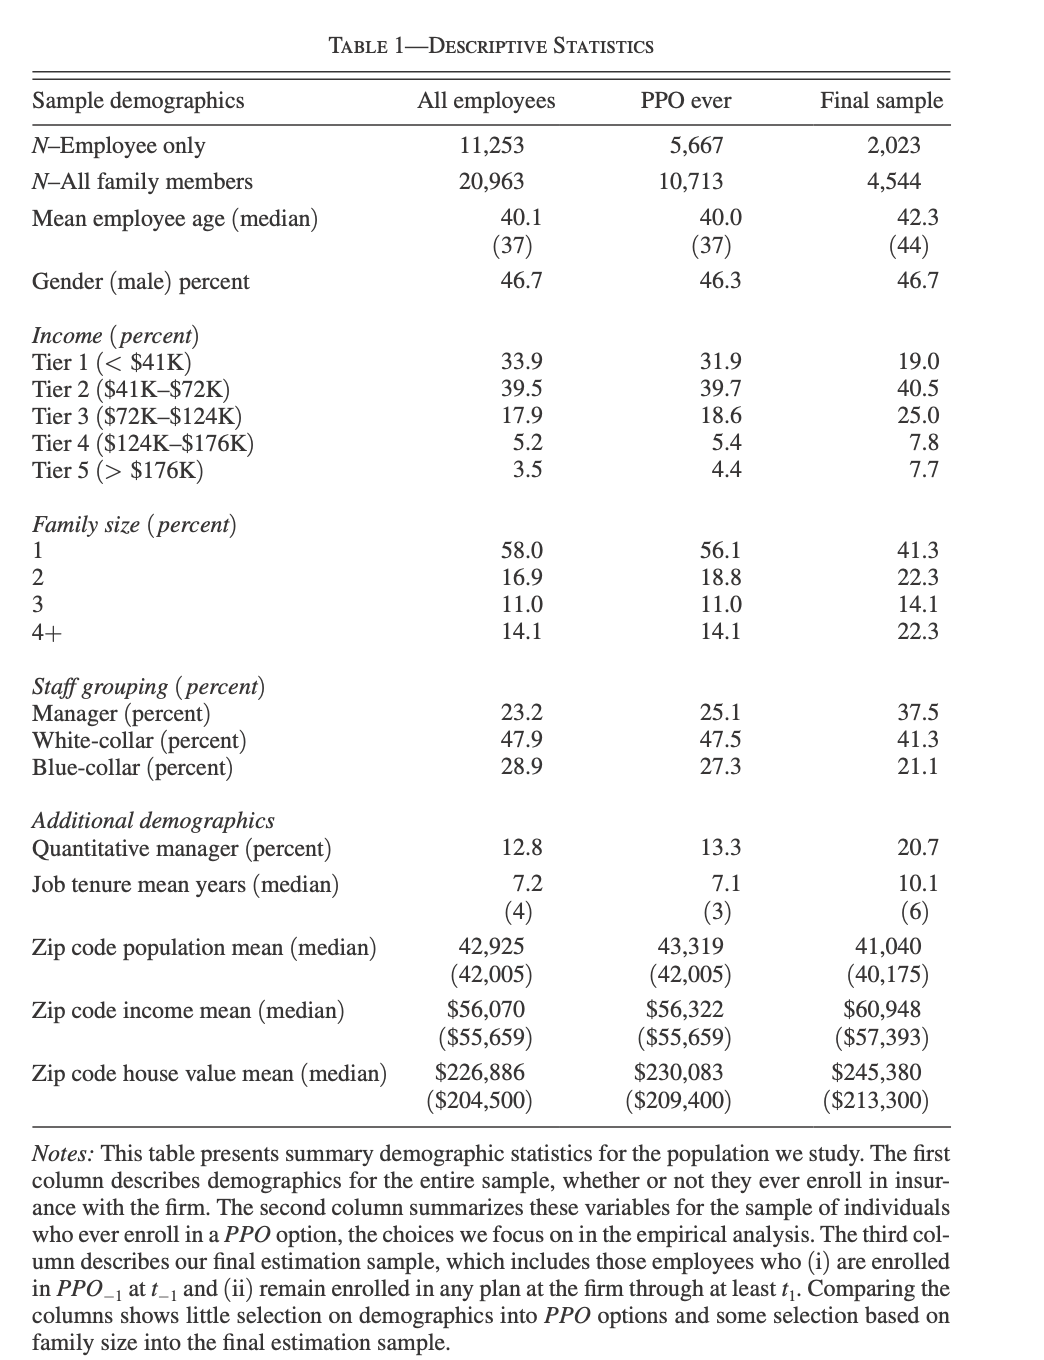
\includegraphics[scale=.3]{resources/handel_t1.png}
\end{center}
\end{frame}


\begin{frame}{How do insurance contracts look?}
\begin{center}
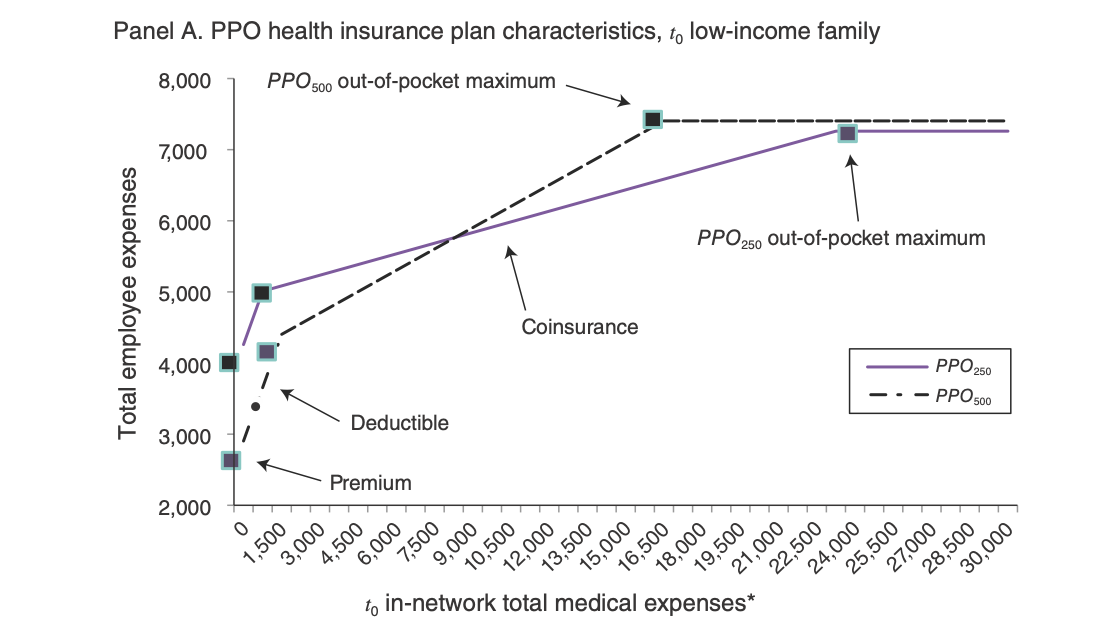
\includegraphics[scale=.37]{resources/handel_f1a.png}
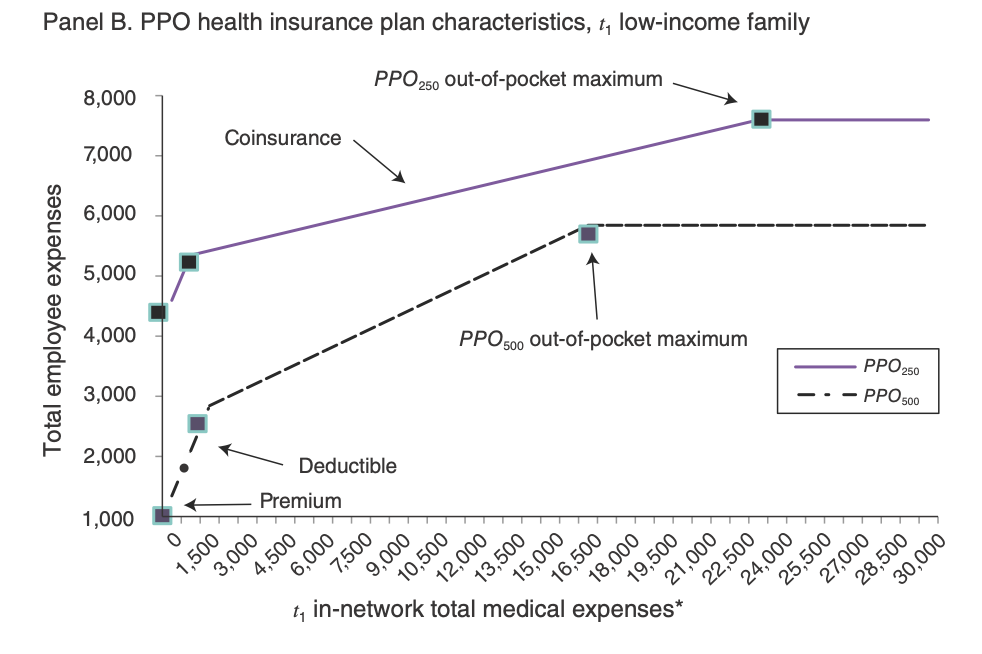
\includegraphics[scale=.37]{resources/handel_f1b.png}
\end{center}
\end{frame}

\begin{frame}{Evolution of Premiums}
\begin{center}
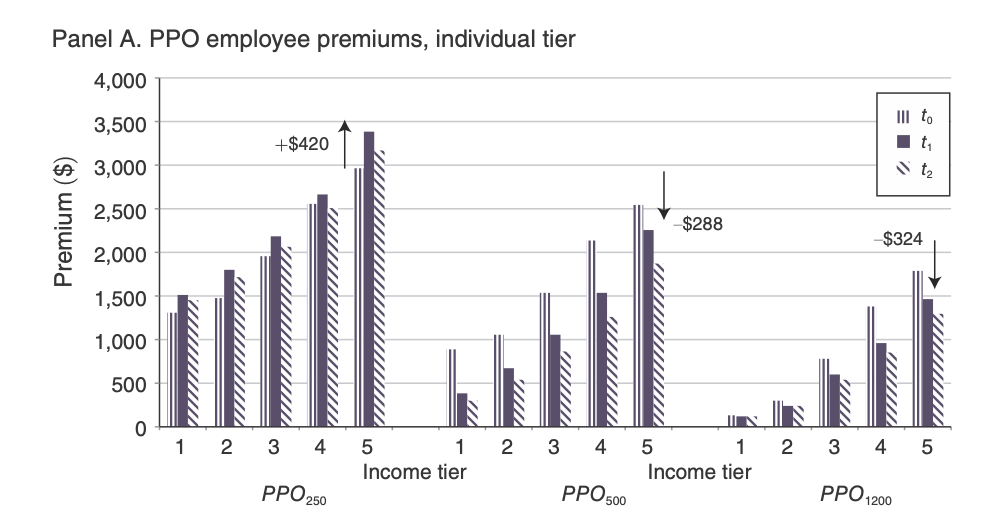
\includegraphics[scale=.37]{resources/handel_f2a.png}
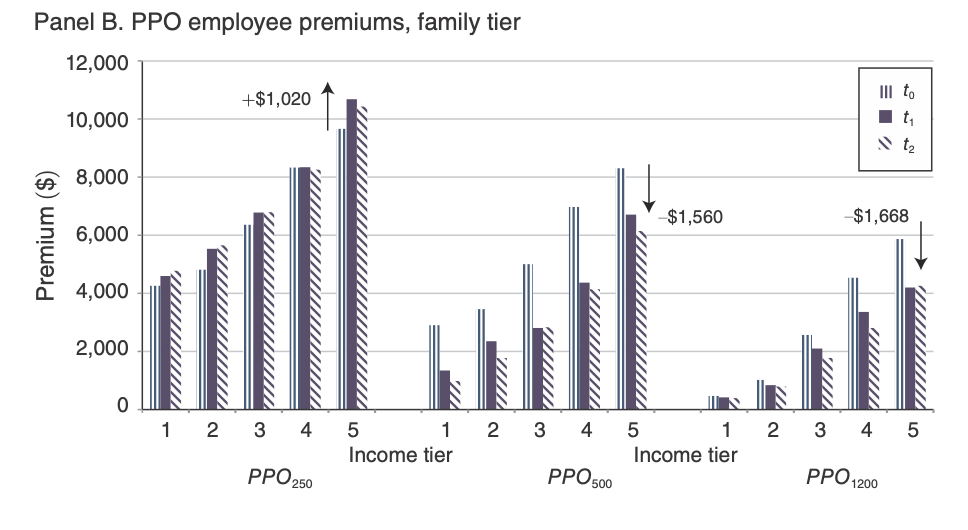
\includegraphics[scale=.37]{resources/handel_f2b.png}
\end{center}
\end{frame}



\begin{frame}
\frametitle{Data: Three Descriptive Tests}
\begin{enumerate}
\footnotesize
\item Compare new employees, who make active choices at coverage at $%
t_{i}$, to prior cohorts who decide whether to change plans at $t_{i}$ (See
KM Ericson 2012).
\begin{itemize}
\footnotesize
\item New entrants similar to prior cohorts in obs demographics
\item Choices of prior cohorts at $t$ reflect choice setting at $%
t_{-1}$.
\item Note: this sample not used for baseline model
\end{itemize}
\item PPO$_{250}$ becomes strictly dominated at $t_{1}$ for some family
size and income groups. 

\begin{itemize}
\footnotesize

\item Only 11\% switch to a non-dominated plan at $t_{1}$; only 25\% of
those remaining switch at $t_{2}$

\item Those who switch are also more likely to switch dental coverage, have
an FSA. 

\item Switchers younger, lower income, male

\item Info shock or unobserved indiv characteristic?
\end{itemize}
\item Test of adverse selection

\begin{itemize}
\footnotesize

\item Look across plans available in all years with the same coverage

\item Find higher health risks chose plans with more comprehensive coverage. 

\item Important for Einav, Finkelstein, Cohen (2010) test: need complete  OOP expenses
\begin{itemize}\footnotesize

\item Time Series data, see premiums increase and little change in risk.
\item Cross-section on same plan provides evidence of adverse selection
\end{itemize}

\end{itemize}
\end{enumerate}
\end{frame}




\begin{frame}{Evidence of Switching Costs: New Employees and Dominated Plan}
\begin{center}
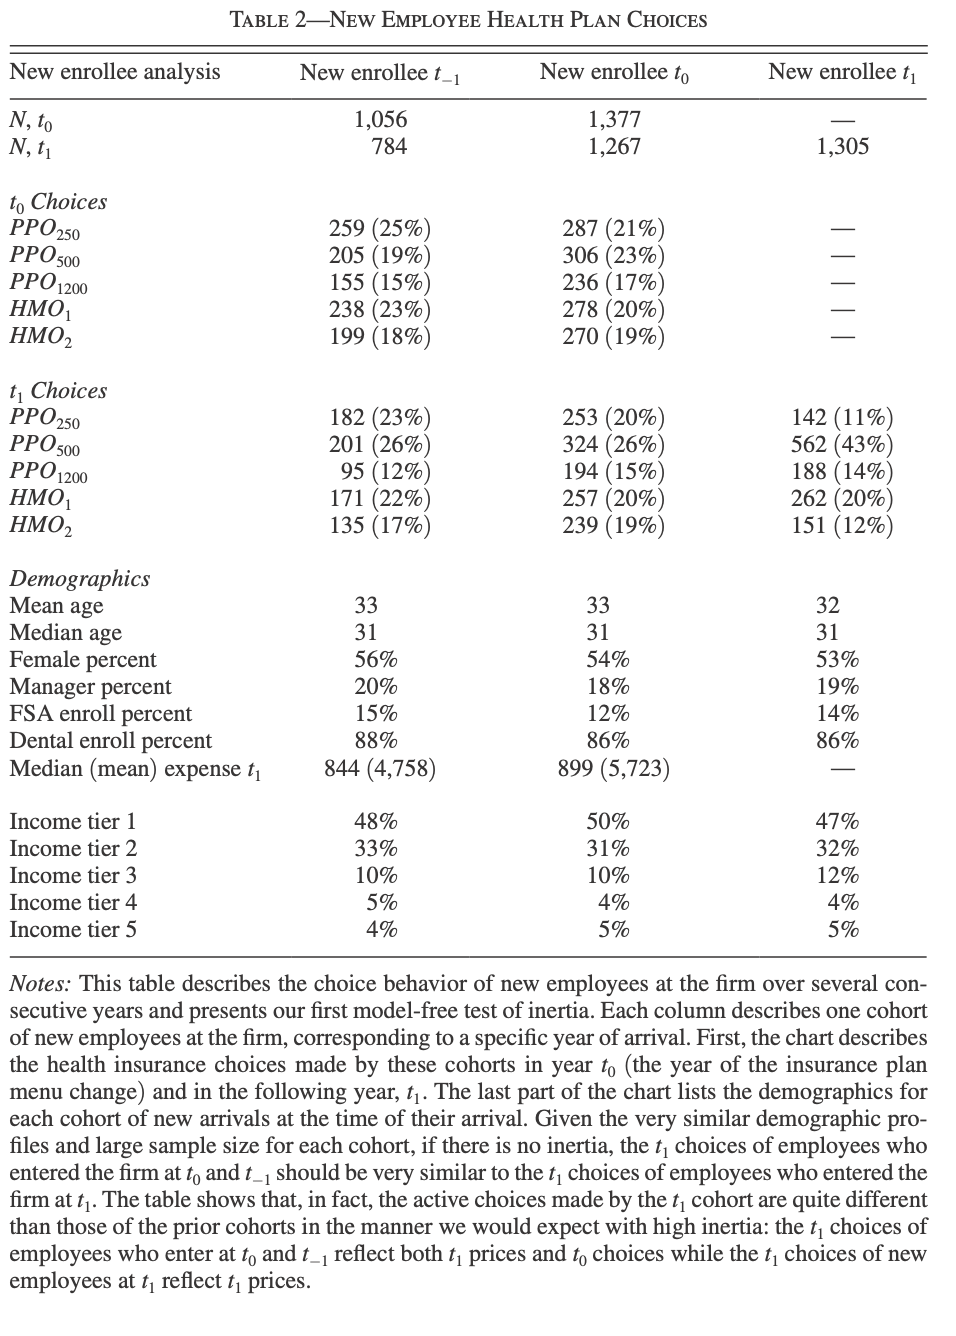
\includegraphics[scale=.3]{resources/handel_t2.png}
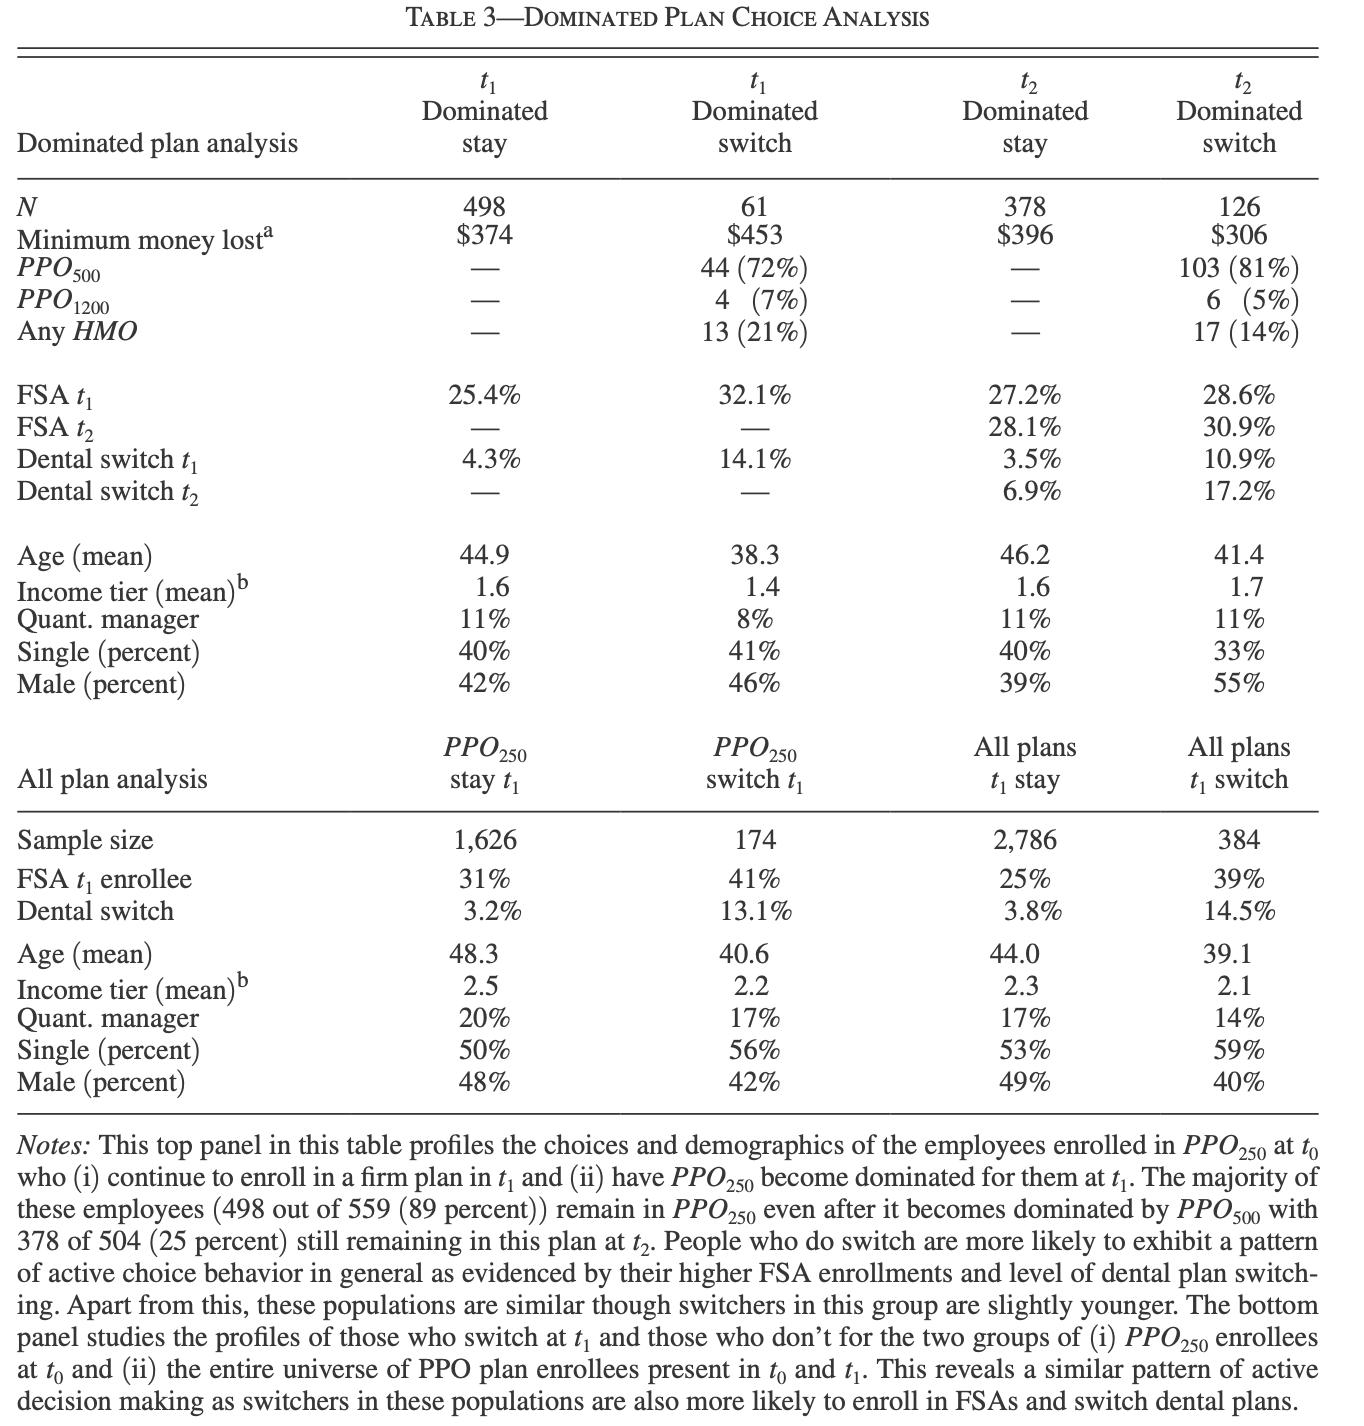
\includegraphics[scale=.3]{resources/handel_t3.png}
\end{center}
\end{frame}


\begin{frame}
\frametitle{Model: Cost model}

\begin{itemize}
\item Assume: (1) consumers' beliefs match the cost model's estimates (no private information), and (2) no moral hazard

\item Procedure to determine $F_{kjt}(.)$
\begin{itemize}
\item Enter past diagnoses and payments in JH model to predict future medical and pharmacy expenditures
\item Divide sample into groups based on predicted expenditures
\item Fit the empirical distrib of ex post claims for each spending category and sample group (allow corr)
\item Map joint distrib of claims to OOP
\end{itemize}

\item Robustness: adjust the output of the cost model to have lower
utilization in less comprehensive plans.

\end{itemize}
\end{frame}



\begin{frame}{Handel: Demand Model}
Use what Einav, Finkelstein, and Levin (2010) call a ``realized'' empirical utility model and assume that $U_{kjt}$ has the following von-Neuman Morgenstern (v-NM) expected utility formulation
\begin{align*}
U_{k j t}&=\int_{0}^{\infty}  u_{k}\left(W_{k}, O O P, P_{k j t}, 1_{k j, t-1}\right) f_{k j t}(O O P) d O O P\\
u_{k}(x)&=-\frac{1}{\gamma_{k}\left(\mathbf{X}_{k}^{A}\right)} e^{-\gamma_{k}\left(\mathbf{x}_{k}^{A}\right)_{x}}
\end{align*}
\begin{itemize}
\item $k$ is a family unit,  $j$ is an insurance plan,  $t$ is a year $(t_0,t_1,t_2)$.
\item $\gamma = \frac{u''(\cdot) }{u'(\cdot)}$ CARA risk-aversion (larger is more risk-averse).
\end{itemize}
\end{frame}


\begin{frame}{Handel: Demand Model}
\begin{align*}
x &=W_{k}-P_{k j t}-O O P+\eta\left(\mathbf{X}_{k t}^{B}, Y_{k}\right) 1_{k j, t-1}+\delta_{k}\left(Y_{k}\right) 1_{1200}+\alpha H_{k, t-1} 1_{250}+\epsilon_{k j t}\left(Y_{k}\right)
\end{align*}
\begin{itemize}
\item $W_k$ family wealth.
\item $P_{k j t}$ is the price for insurance plan $j$ to family $k$.
\item $OOP$ is a draw from the distribution of $f(OOP)$ expenses: depends on the plan.
\item $\eta\left(\mathbf{X}_{k t}^{B}, Y_{k}\right) 1_{k j, t-1}$ is the switching cost which depends on demographics $\mathbf{X}_{k t}^{B}$.
\item $\delta_{k}(Y_k)$ is the family specific intercept for high-deductible plan $(Y_k)$ is family dummy.
\item $\alpha H_{k, t-1} 1_{250}$ is interaction between 90th percentile spenders and most generous plan.
\end{itemize}
\end{frame}

\begin{frame}
\frametitle{Supply Model}



\begin{itemize}
\item Total premium set as average plan cost for the plan's enrollees in
prior year plus administrative markup (and conditional on income/family
level, $y$):%
\begin{align*}
TP_{jt}^{y}=AC_{K_{j,t-1}^{y}}+L=\frac{1}{||K_{j,t-1}^{y}||}\sum_{k\in
K_{j,t-1}^{y}}PP_{kj,t-1}+L
\end{align*}
\item Subsidy to employee as a percentage of PPO$_{1200}$ premium
\end{itemize}
\end{frame}

\begin{frame}
\frametitle{Identification}

\begin{itemize}
\item Identify consumer preference heterogeneity using choices from the
forced re-enrollment period

\item Identify switching costs by analyzing how choices change over time as
predicted active plan values change.

\item Identify preference for PPO$_{1200}$ HSA by looking at choice of nest
\{PPO$_{250}$,PPO$_{500}$\} vs. \{PPO$_{1200}$\}.
\end{itemize}
\end{frame}

%--------------------------------------------------------------------------------

\begin{frame}
\frametitle{Estimation}

\begin{itemize}
\item Normal distribution on random coefficients:%
\begin{eqnarray*}
\gamma _{k}(X_{k}^{A}) &\backsim &N(\mu _{\gamma }(X_{k}^{A}),\sigma
_{\gamma }^{2}) \\
\mu _{\gamma }(X_{k}^{A}) &=&\mu +\beta (X_{k}^{A})
\end{eqnarray*}

\item Switching costs:%
\begin{align*}
\eta (X_{k}^{B},Y_{k})=\eta _{0}+\eta _{1}X_{kt}^{B}+\eta _{2}Y_{k}
\end{align*}

\item Probit error, $\varepsilon _{kjt}$ distributed iid with parms $(\mu
_{\varepsilon _{j}}(Y_{k}),\sigma _{\varepsilon _{j}}(Y_{k}))$

\item Proceed via random coefficients probit SMLE
\end{itemize}
\end{frame}

\begin{frame}
\frametitle{Results : Choice Model}

\begin{itemize}
\item Switching costs \$1729 for singles, \$2480 for family with dependent.
Why--family has more money at stake?

\item Demographics?

\begin{itemize}
\item Enroll in FSA - \$551 lower switching cost

\item Manager -- higher SC; no effect from quant manager

\item Higher SC for chronic patients, those with salient change in medical
history?
\end{itemize}

\item Risk aversion

\begin{itemize}
\item Moderate: 50\% gain \$100, 50\% lose \$92.2. Little heterogeneity
(contrast with Einav and Cohen (2007))

\item Increasing in age and income?

\item Heterogeneity larger in robustness with log-normal risk parameter
\end{itemize}

\item Distaste for HSA
\end{itemize}
\end{frame}

%--------------------------------------------------------------------------------

\begin{frame}
\frametitle{Results: Counterfactuals}

\begin{itemize}
\item Reduce switching costs by multiplicative factor $Z$.  As $Z$ approaches $0$, full optimization in each period.
\item Welfare measure

\begin{itemize}
\item CS is difference in certainty equivalents, for a given family, between the health plan chosen before/after intervention
\item TS differs from CS only if the sum of employees contributions differs in counterfactual scenario
\end{itemize}

\item Naive
\begin{itemize}
\item $3/4$ reduction in switching costs at $t_{2}$: improves consumer choices, $\$114$ mean increase in population; $\$196$ for switchers only.  $5.8\%$ improvement overall.
\end{itemize}
\end{itemize}

\end{frame}

%--------------------------------------------------------------------------------

\begin{frame}
\frametitle{Results: Counterfactuals}

With endogenous price changes:
\begin{itemize}
\item Unravelling: when switching costs reduced, initial switchers are healthier (see reduced form); adverse selection results.
\item With $3/4$ reduction in switching costs: 

\begin{itemize}
\item improves consumer choices conditional on prices
\item worsens adverse selection; ``death spiral" for $PPO_{250}$
\end{itemize}


\item Welfare falls per year, on average by \$115 or 7.7\% (loss from adverse selection without info provision is 8.2\%)
\begin{itemize}
\item Switchers gain \$186/yr (12\% of premiums)
\item Non-switchers lose \$442, due to adverse selection.
\item Distributional effects by demographics (harder to interpret)
\item With switching costs in welfare measure, still see loss
\end{itemize}
\end{itemize}
\end{frame}

%--------------------------------------------------------------------------------
\begin{frame}{Counterfactual Evolution of Plans}
\begin{center}
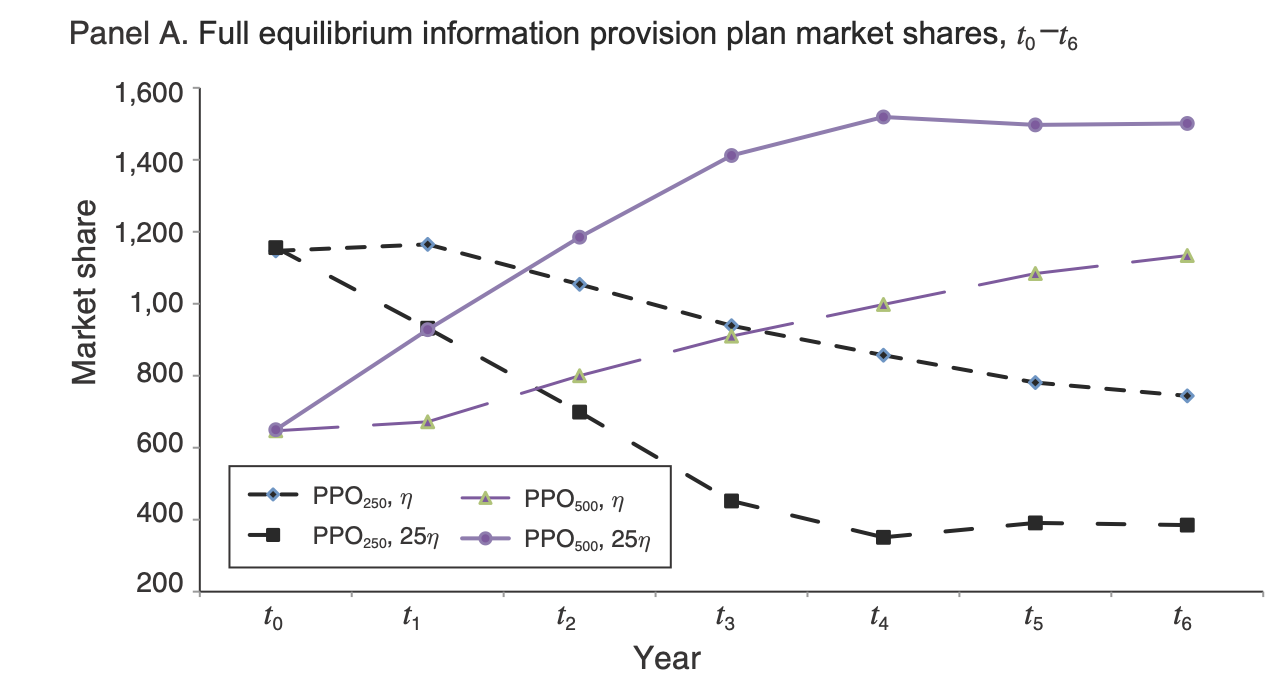
\includegraphics[scale=.3]{resources/handel_f3a.png}
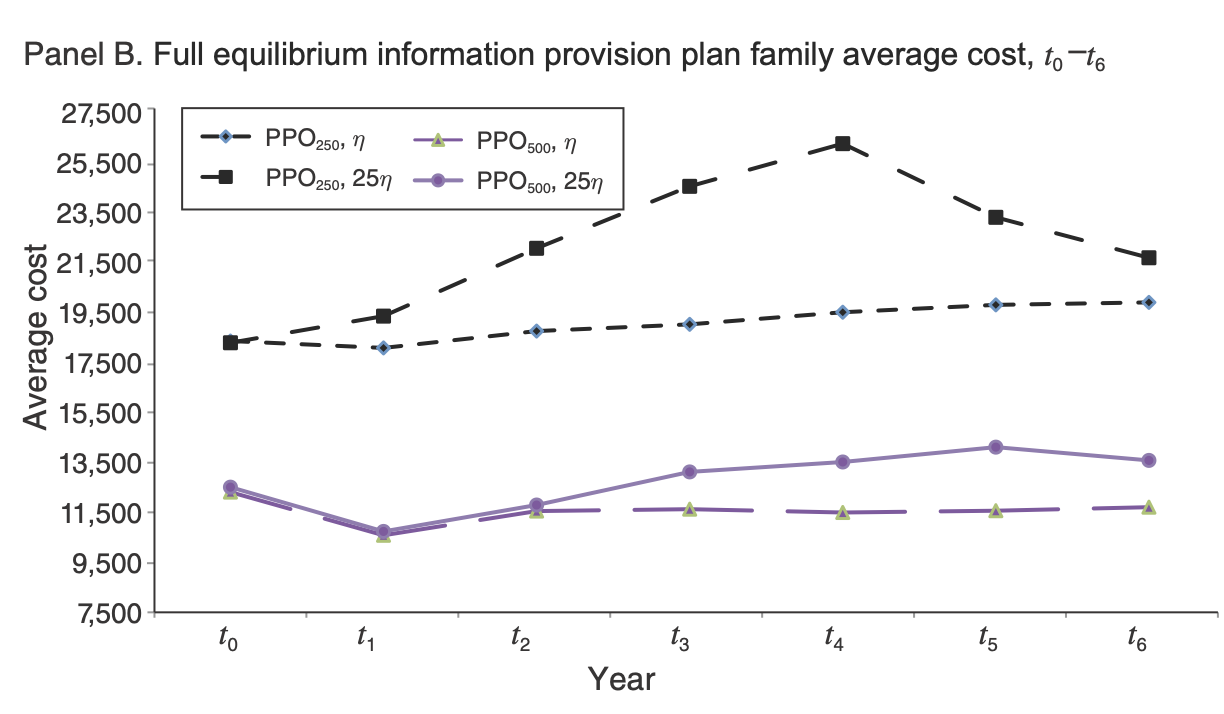
\includegraphics[scale=.3]{resources/handel_f3b.png}
\end{center}
\end{frame}

%--------------------------------------------------------------------------------

\begin{frame}{Counterfactual Evolution of Plans}
\begin{center}
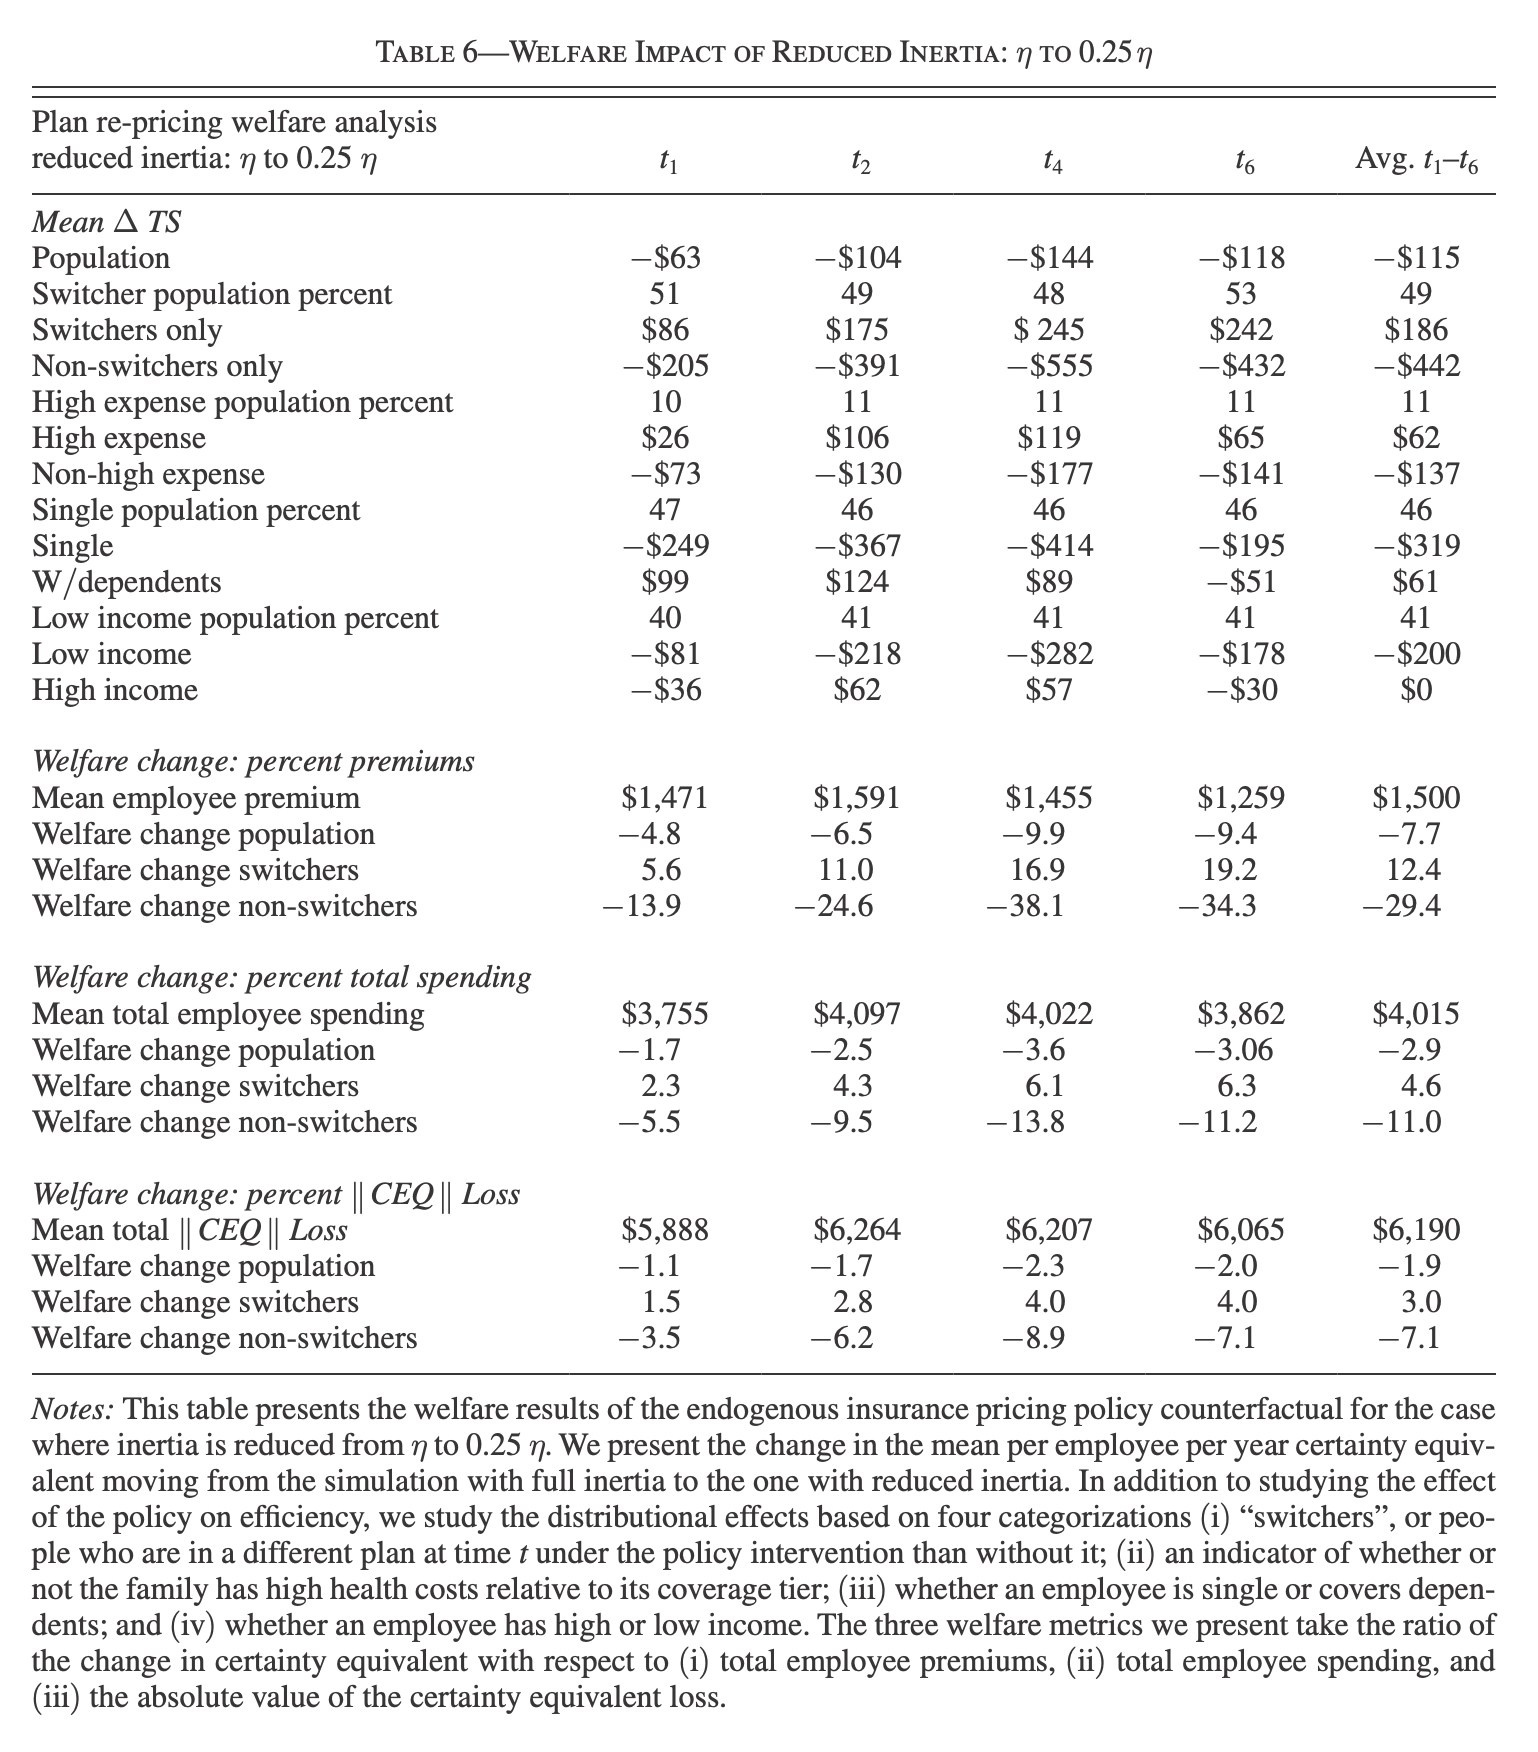
\includegraphics[scale=.3]{resources/handel_t6.png}
\end{center}
\end{frame}


\begin{frame}{Counterfactual Welfare}
\begin{center}
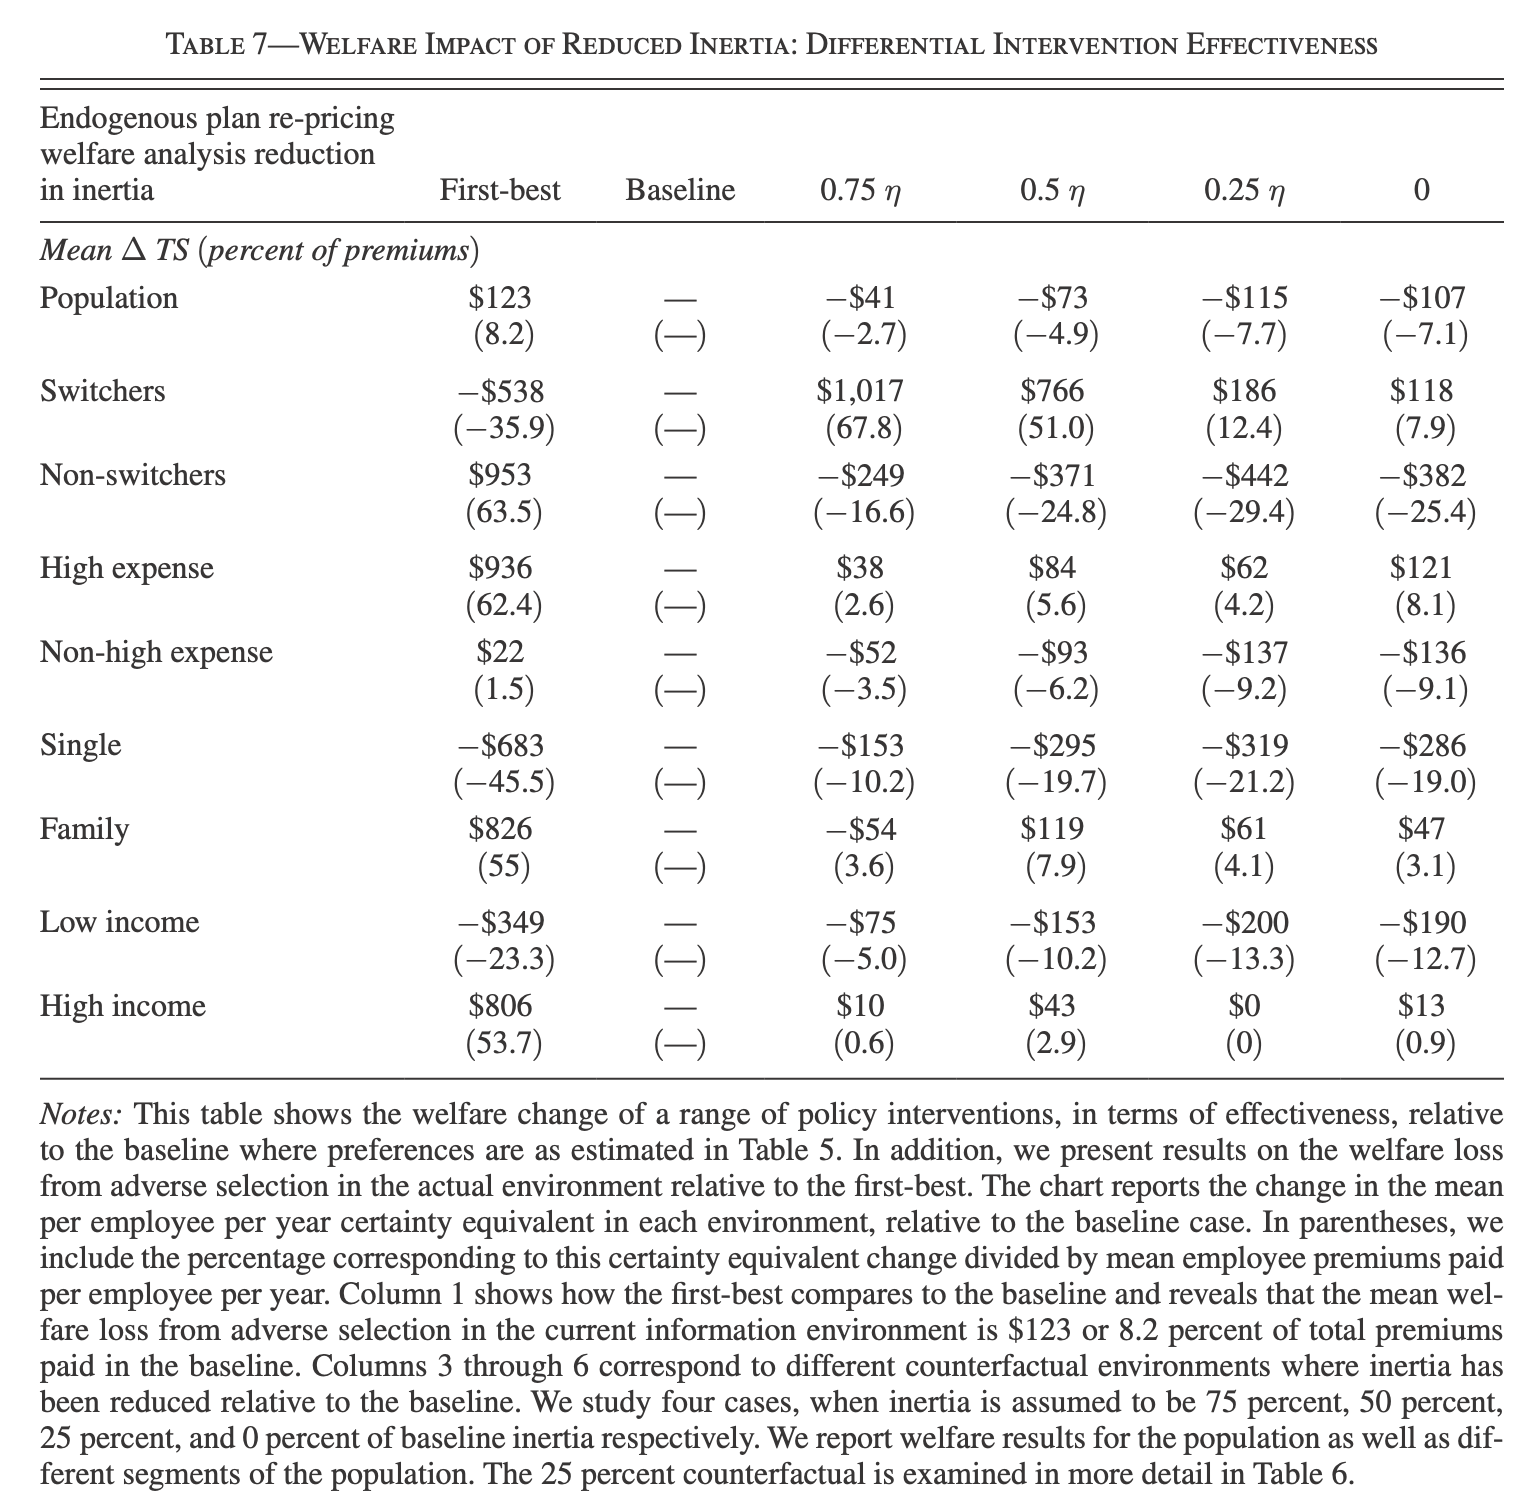
\includegraphics[scale=.3]{resources/handel_t7.png}

\end{center}
\end{frame}


\begin{frame}{Inertia Costs: Real or Psychological?}
\begin{center}
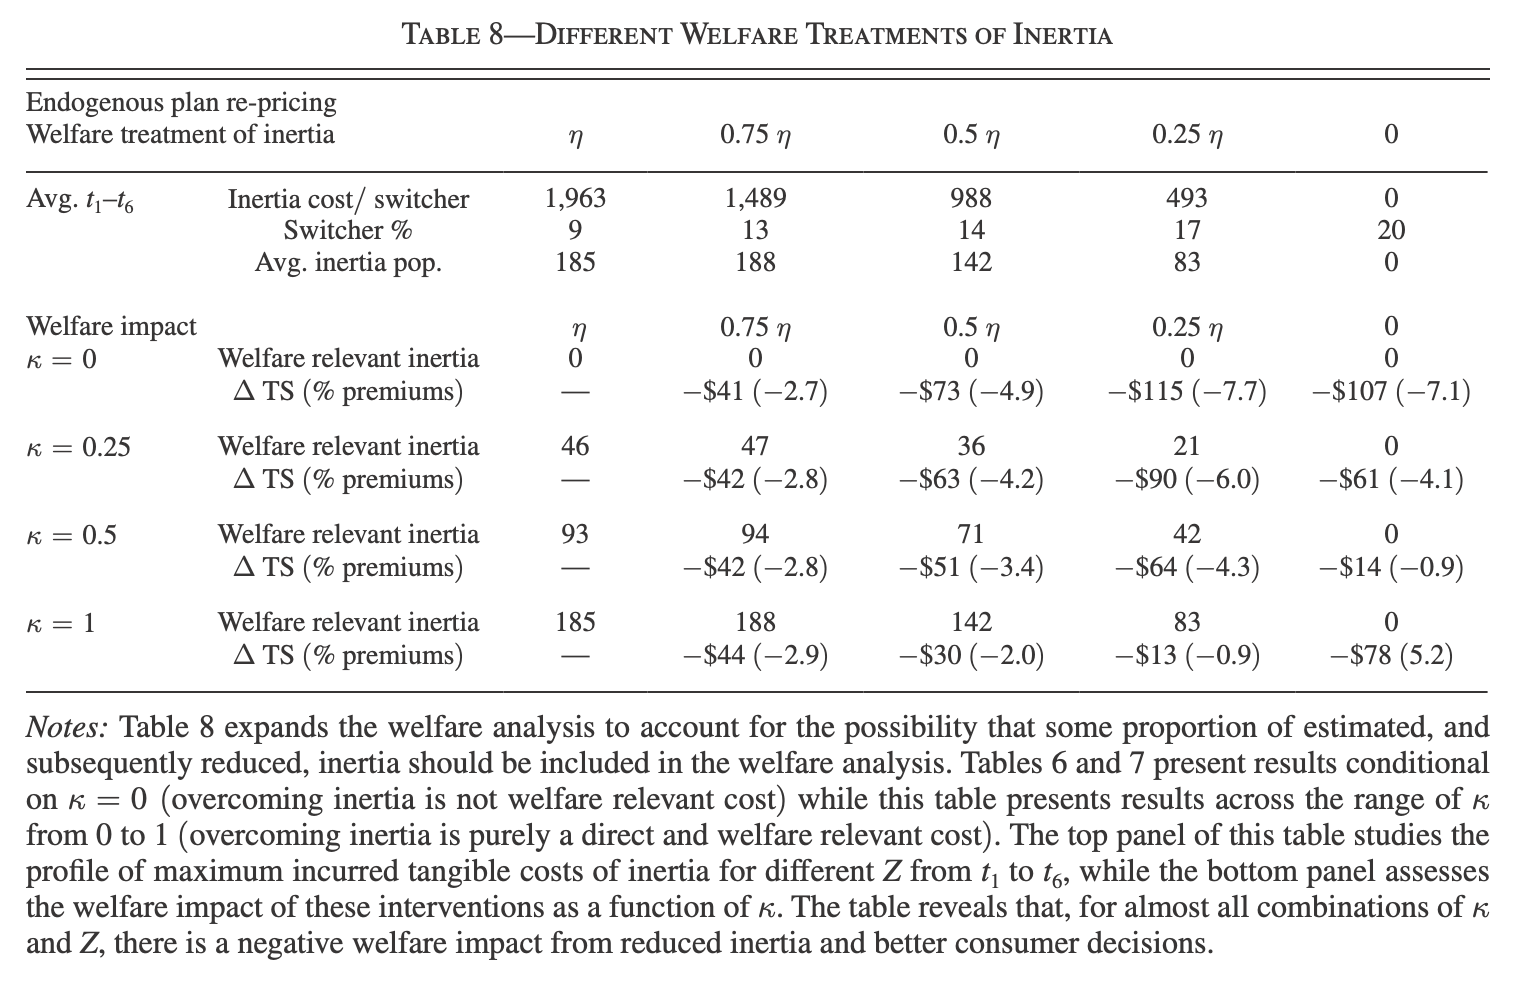
\includegraphics[scale=.5]{resources/handel_t8.png}

\end{center}
\end{frame}


\begin{frame}
\frametitle{Comments: Switching Costs}


\begin{itemize}
\item What is a switching cost?
\begin{itemize}
\item Transaction costs (then SC=0 when no switch)
\item Learning costs  -  effort needed to learn about new plan�s features.
\item Product compatibility - important if network changes (need to make new relationship-specific investments)
\item Fixed re-optimization costs - some cost to changing beliefs from status quo
\item Inertial and psychological costs
\end{itemize}

\item First three are social costs.
\end{itemize}
\end{frame}

%--------------------------------------------------------------------------------

%--------------------------------------------------------------------------------

\begin{frame}
\frametitle{Comments: Can we tell apart stories?}

\begin{itemize}
\item If it's inertia, fixed optimization, then people who switch would have medical costs similar to population
\item If transaction costs, more money at stake would imply more switching.
\item Use of balanced panel: miss a lot of information from new entrants vs. prior cohorts?
\end{itemize}
\end{frame}

%--------------------------------------------------------------------------------

%--------------------------------------------------------------------------------

\begin{frame}
\frametitle{Comments: Implications for insurance design}


\begin{itemize}
\item Keep consumers uninformed to prevent adverse selection from worsening?
\item Information opaqueness an alternative to mandates?
\item Use risk adjustment along with info provision.
\begin{itemize}
\item Continue lump sum subsidies (consumers face the marginal price of their choice)
\item Transfers/risk-adjustment prevent death spiral from adverse selection under AC-pricing
\end{itemize}

\end{itemize}


\end{frame}

%--------------------------------------------------------------------------------

\begin{frame}
\frametitle{Comments: Endogeneity question}

\begin{itemize}
\item Firms respond to stickiness using introductory pricing, advertising, etc
\item Consumer stickiness built by ``endogenous sunk costs" (Sutton)--network formation, brand loyalty,...
\end{itemize}

\end{frame}


\begin{frame}
\frametitle{Aside: Researchable Topics}

Questions we might ask:
\begin{itemize}
\item How are prices set?
\item Ratcheting effect from non-durable good due to information revelation?
\item Do firms exploit 'inertia' of consumers in their pricing decisions?
\begin{itemize}
\item In theory literature, 'invest then harvest' pricing
\item Or is it another form of price discrimination?
\item How big are switching costs- both pecuniary and non-pecuniary- in Part D plans? ESI plans?
\end{itemize}
\end{itemize}
\end{frame}
%--------------------------------------------------------------------------------

\begin{frame}
\frametitle{Aside: Researchable Topics}

Questions we might ask:
\begin{itemize}
\item Firms prohibited from pricing new vs. continuing enrollees differently.  Can the firm use contract proliferation as a means to accomplish the same goal?
\item What explains the choice in the initial period for a plan with a higher premium? 
\item Are profits higher in the plans with greater enrollment? Cream-skimming strategy?
\end{itemize}
\end{frame}



\end{document}













































